\begin{frame}
\frametitle{Regularized potential}
\scriptsize

Extracting an \emph{analytical} cusp from the wave function
\footcite{Bischoff_2014a}
\begin{itemize}
    \item Nuclear correlation factor $R$
    \item Numerical exponential molecular orbital (NEMO)\footcite{Seelig_1966} $F_i$
\end{itemize}

\vspace{5mm}

\centering
\textbf{Wave function ansatz}
\begin{equation}
    \nonumber
    \ket{\phi_i} = R\ket{F_i}
\end{equation}

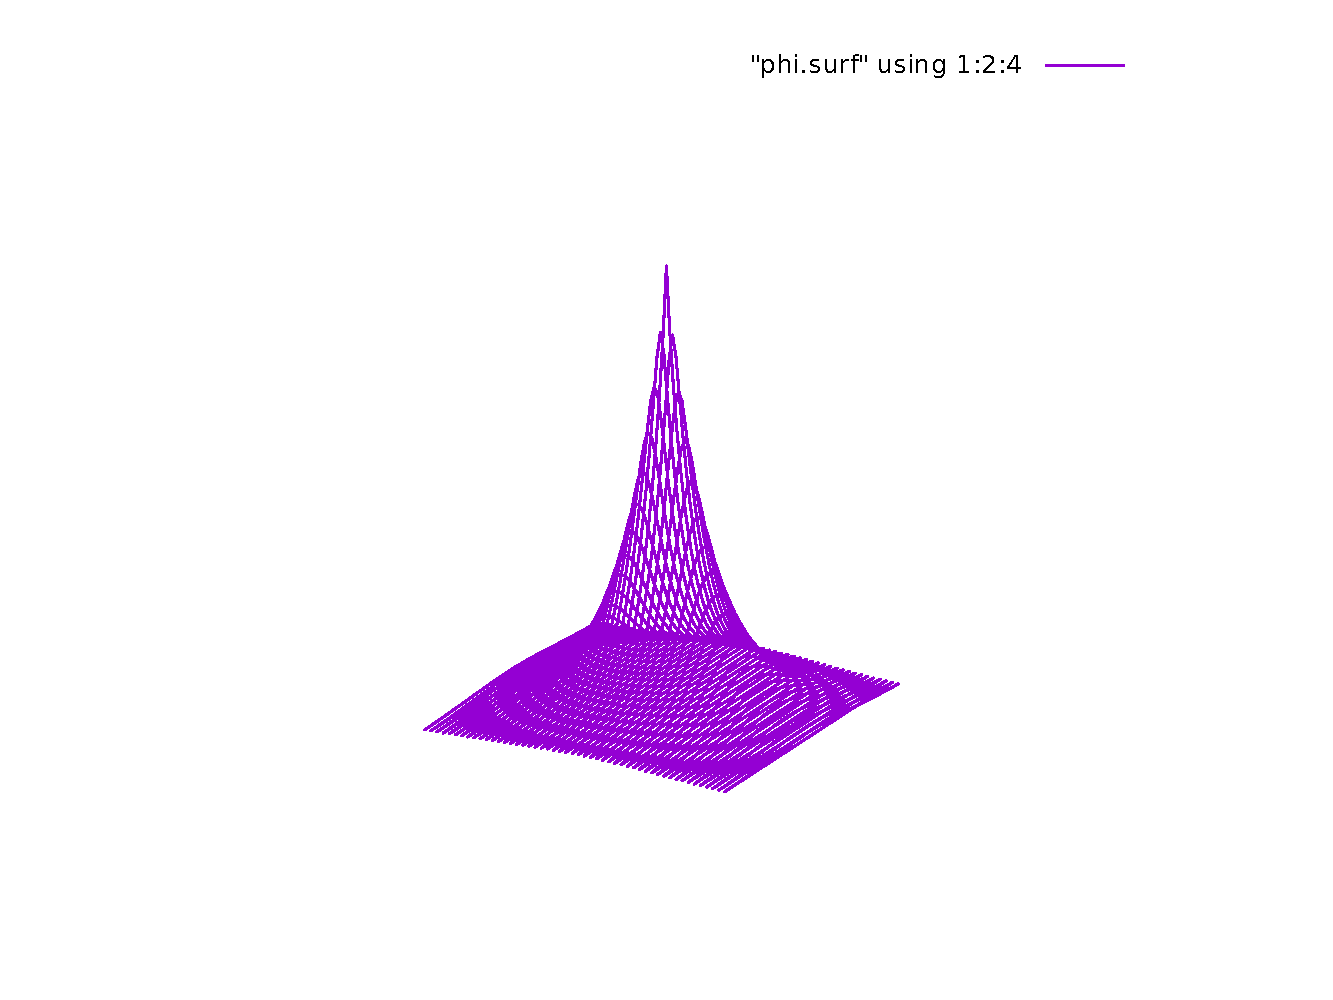
\includegraphics[scale=0.35, viewport = 175 90 430 400, clip]{figures/phi.pdf}
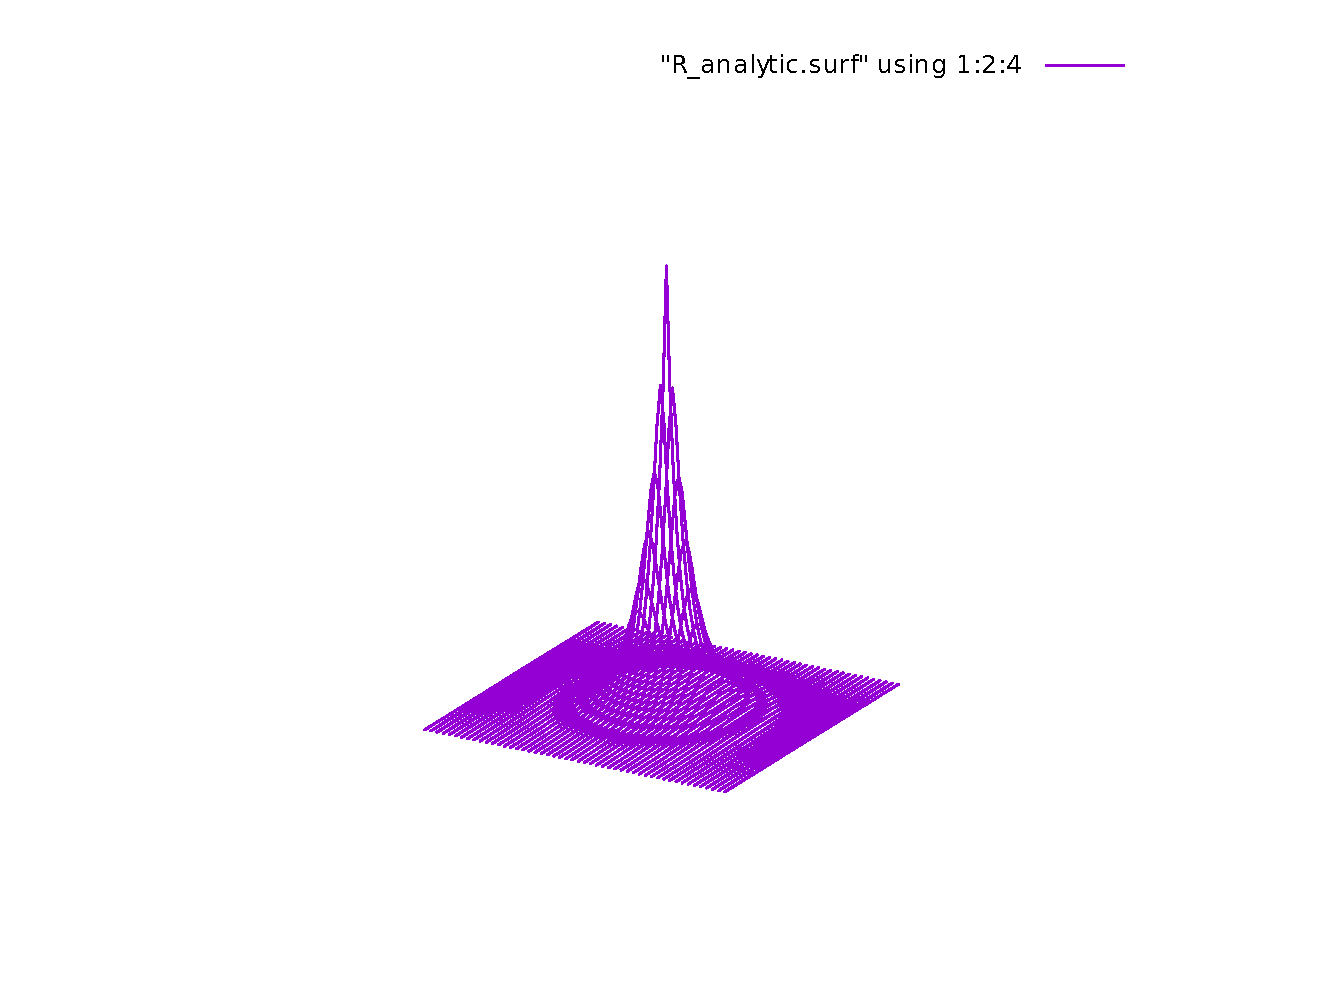
\includegraphics[scale=0.35, viewport = 175 90 430 400, clip]{figures/R.pdf}
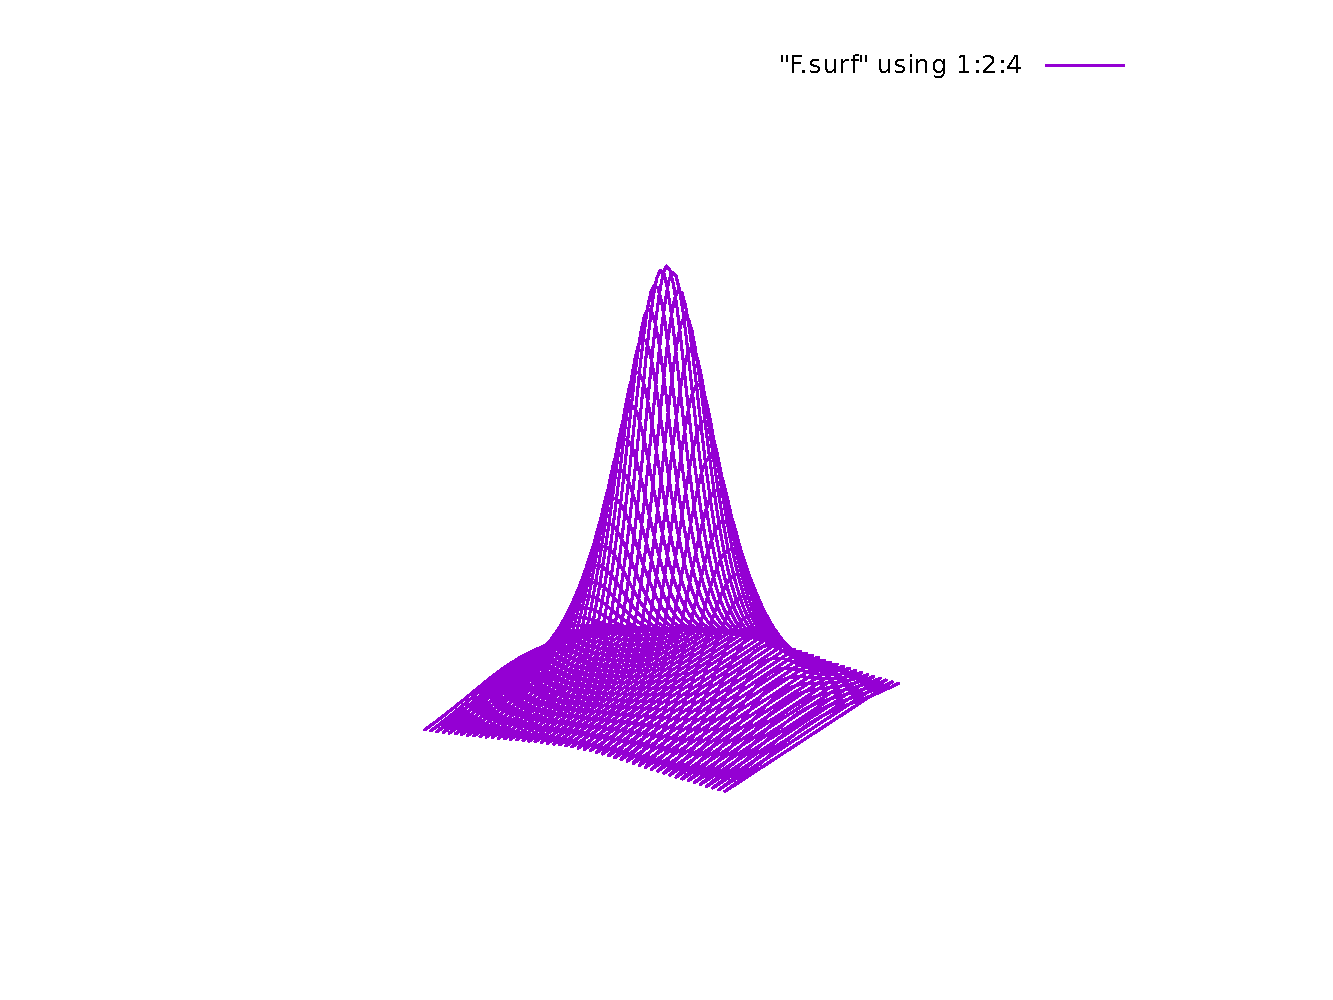
\includegraphics[scale=0.35, viewport = 175 90 430 400, clip]{figures/F.pdf}\\

\end{frame}

\begin{frame}
\frametitle{Regularized potential}
\scriptsize
\centering

\textbf{Hartree-Fock equations}
\begin{equation}
    \nonumber
    \Big(T + V_{nuc} + J - K - \epsilon_i\Big)R\ket{F_i} = 0
\end{equation}

\vspace{5mm}

\pause
\textbf{Commuting the correlation factor to the left}
\begin{equation}
    \nonumber
    R\Big(T + R^{-1}[T,R] + V_{nuc} + J - R^{-1}KR - \epsilon_i\Big)\ket{F_i} = 0
\end{equation}

\vspace{5mm}

\pause
\textbf{Similarity transformed equations}
\begin{equation}
    \nonumber
    \Big(T + U_{nuc} + J - K_R - \epsilon_i\Big)\ket{F_i} = 0
\end{equation}
\begin{equation}
    \nonumber
    U_{nuc} = V_{nuc} + R^{-1}[T,R]
\end{equation}
\begin{equation}
    \nonumber
    K_R = R^{-1}KR
\end{equation}

\end{frame}

\usebackgroundtemplate{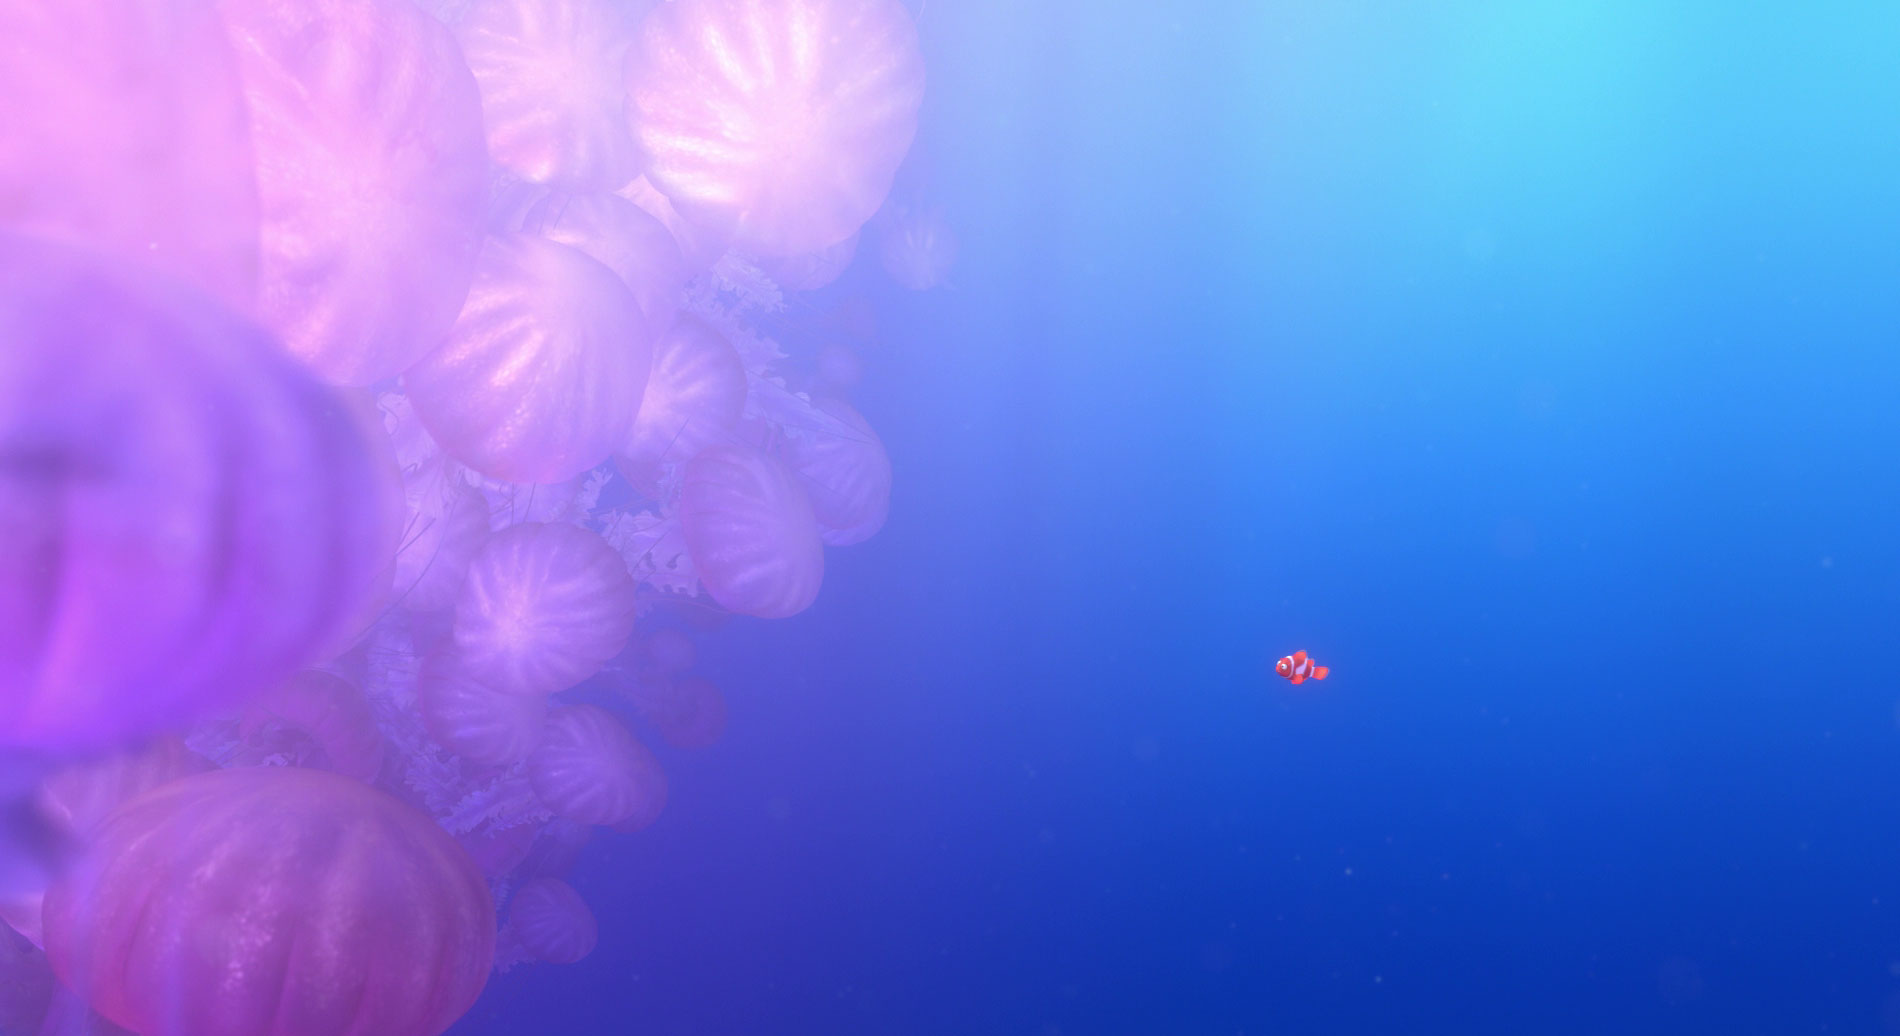
\includegraphics[scale=0.45, viewport=550 280 1400 900, clip]{figures/nemo_background.jpeg}}

\begin{frame}
\frametitle{Finding NEMO}
\scriptsize

\centering
\textbf{Transformed nuclear potential}
\centering
\begin{align}
    \nonumber
    U_{nuc} &=  V_{nuc} + R^{-1}[T,R]
             =  \Big(-\frac{Z}{r}\Big) + \Big(- \frac{\vec{R}^{'}}{R}\cdot\vec{\nabla}
                -\frac{1}{2}\frac{R^{''}}{R}\Big)
\end{align}

\vspace{5mm}

\begin{columns}
\begin{column}{.5\textwidth}

\pause
\centering
\only<1>{

\vspace{42.5mm}

}
\only<2,3,4>{
\textbf{Seelig's NEMO}
\begin{align}
    \nonumber
    R &= e^{-Zr}\\
    \nonumber
    -\frac{\vec{R}^{'}}{R} &= Z\vec{n}\\
    \nonumber
    -\frac{R^{''}}{R} -\frac{Z}{r} &= Z^2
\end{align}
}

\vspace{5mm}

\pause
\only<2>{

\vspace{12.5mm}

}
\only<3,4>{
\textbf{Regularized potential}
\begin{align}
    \nonumber
    U_{nuc} &=  Z\vec{n}\cdot\vec{\nabla} + \frac{Z^2}{2}
\end{align}
}
\end{column}

\begin{column}{.5\textwidth}
\centering
\only<4>{
\textbf{Slater NEMO}
\begin{equation}
    \nonumber
    R = 1 + \frac{e^{-aZr}}{a-1}
\end{equation}

\vspace{3mm}

\textbf{Gauss-Slater NEMO}
\begin{equation}
    \nonumber
    R = e^{-Zr} + \big(1 - e^{-Z^2r^2}\big)
\end{equation}

\vspace{3mm}

\textbf{Polynomial NEMO}
\begin{equation}
    \nonumber
    R = 1 + (-1)^na(-1+rZ/b)^n
\end{equation}
}

\end{column}
\end{columns}

\end{frame}

\usebackgroundtemplate{
\includegraphics[width=1.02\paperwidth]{figures/ctcc_general.jpg}}

\begin{frame}
\frametitle{Hydrogen atom}
\scriptsize

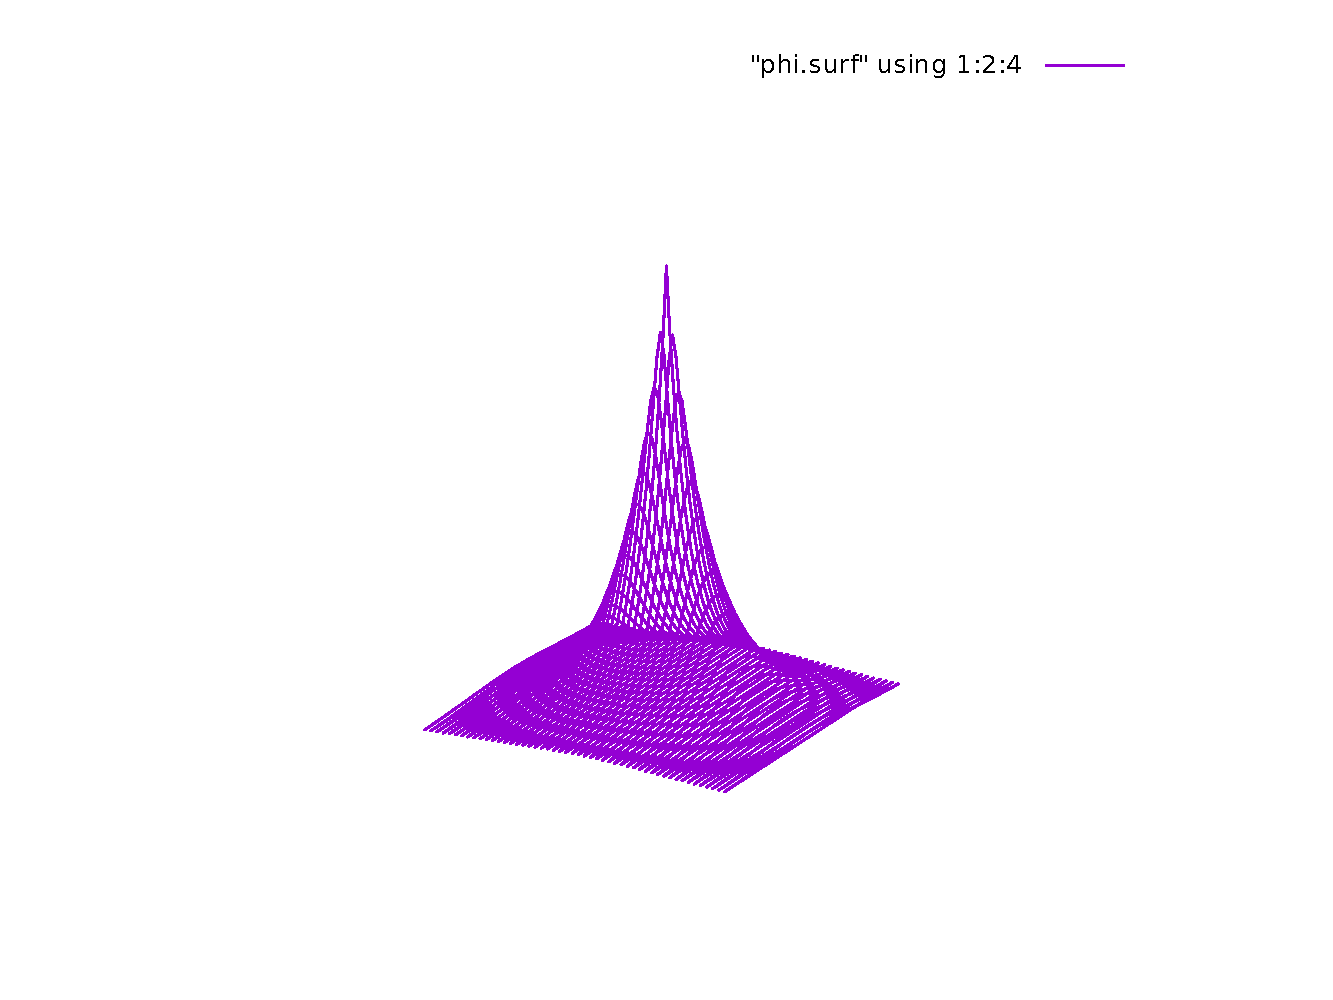
\includegraphics[scale=0.35, viewport = 175 90 430 400, clip]{figures/phi.pdf}
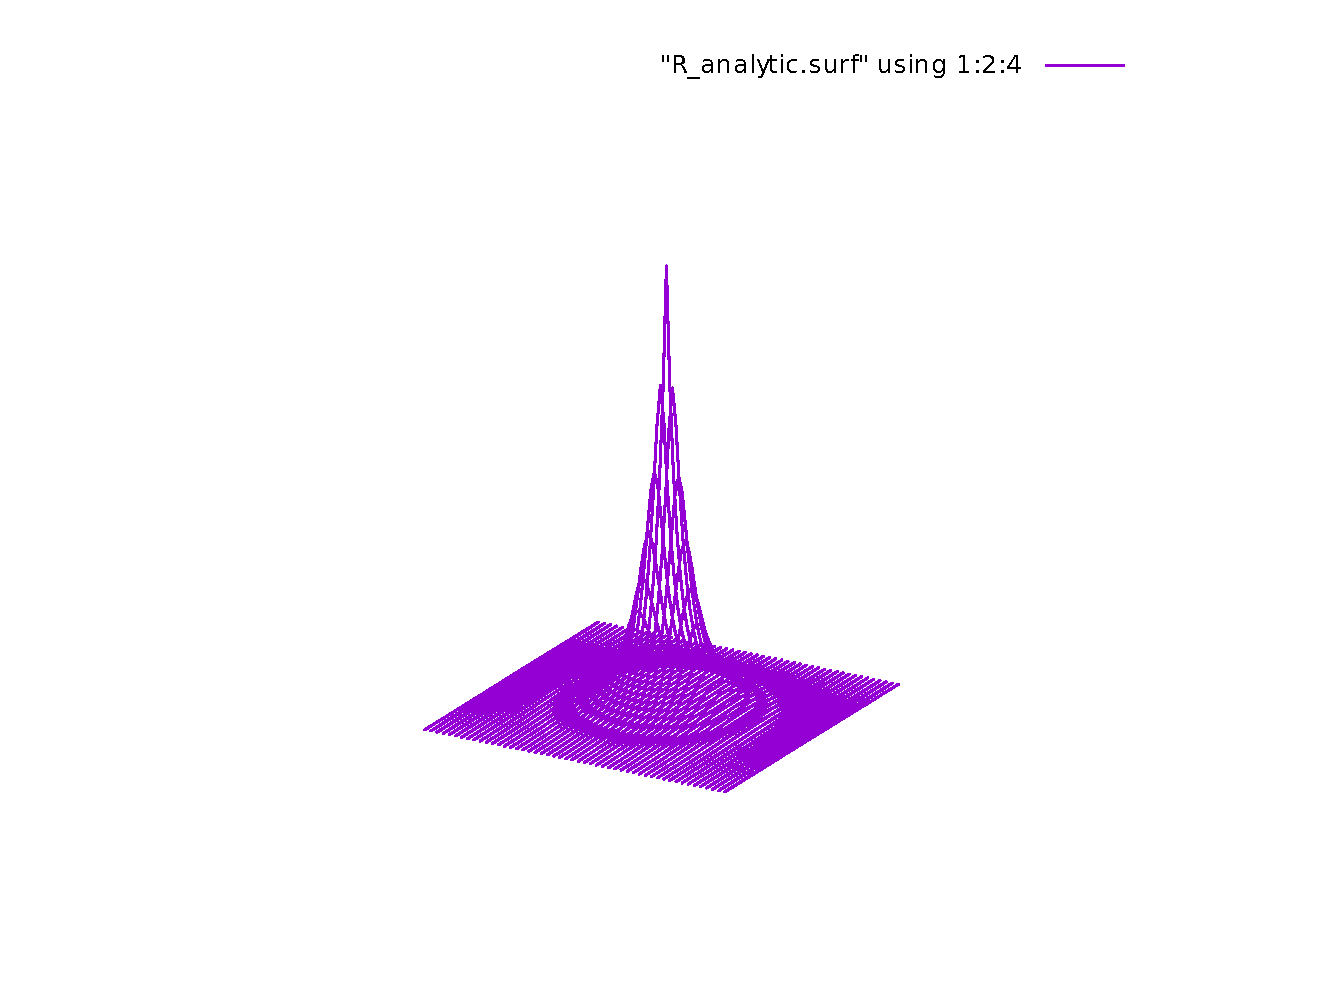
\includegraphics[scale=0.35, viewport = 175 90 430 400, clip]{figures/R.pdf}
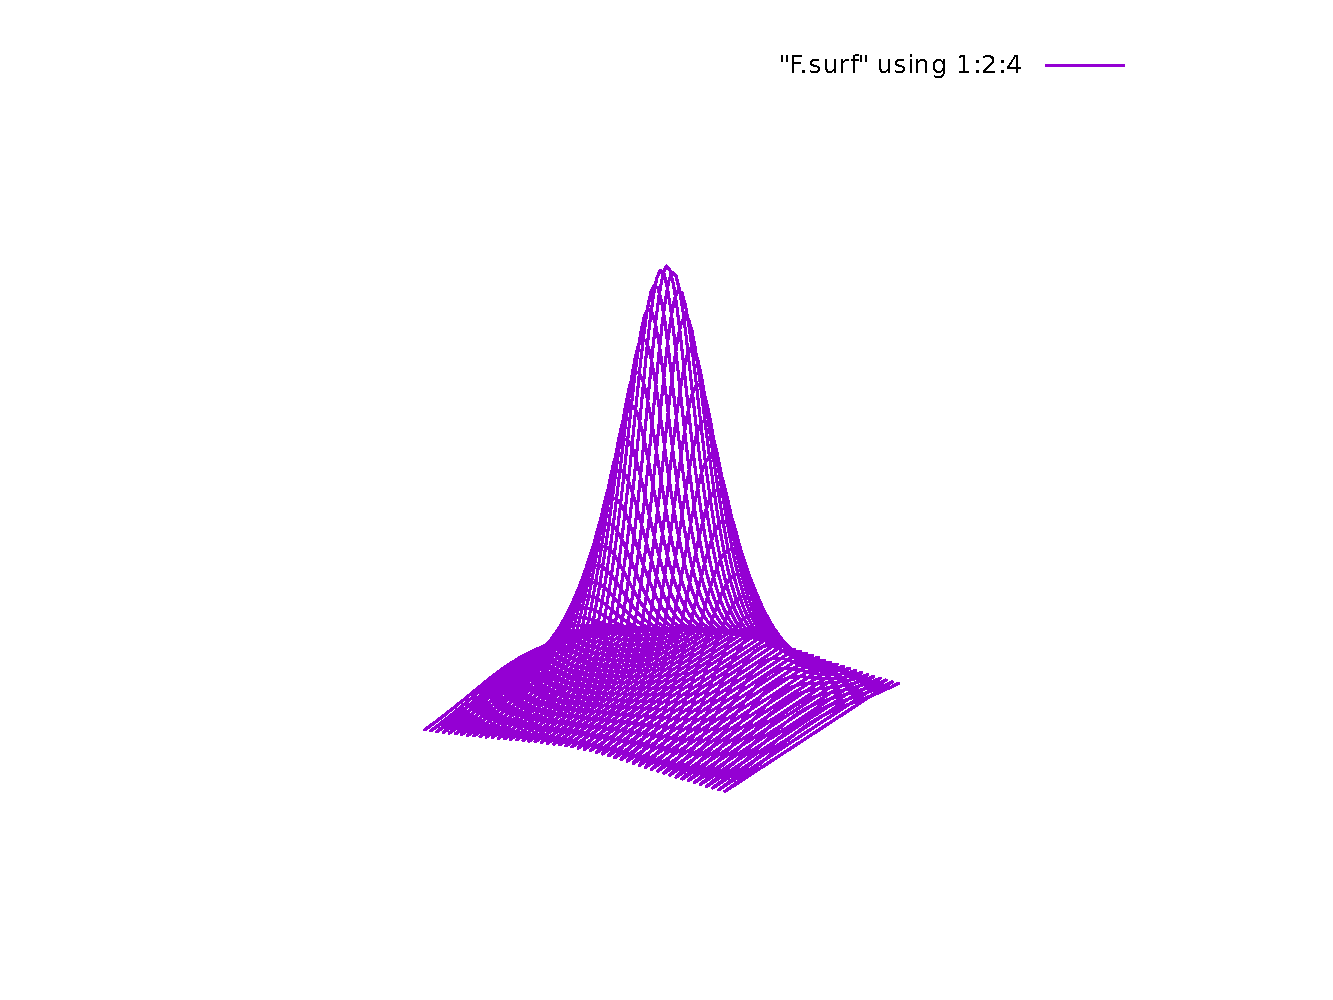
\includegraphics[scale=0.35, viewport = 175 90 430 400, clip]{figures/F.pdf}\\

\begin{table}
\begin{tabular}{ccccccc}
\hline
\hline
Precision&
\multicolumn{1}{c}{\ }&
\multicolumn{1}{c}{$\phi(r_0)$}&
\multicolumn{1}{c}{$\phi(r_1)$}&
\multicolumn{1}{c}{\ }&
\multicolumn{1}{c}{$\phi(r_0)$}&
\multicolumn{1}{c}{$\phi(r_1)$}\\
\hline
\hspace{5mm}\ &\hspace{1mm}\ &\hspace{15mm}\ &\hspace{15mm}\ &\hspace{2mm}\ &\hspace{15mm}\ &\hspace{15mm}\ \\
&\multicolumn{1}{c}{\ }
&\multicolumn{2}{c}{R = Identity}                          
&\multicolumn{1}{c}{\ }
&\multicolumn{2}{c}{\ }\\                          
$\epsilon = 10^{-4}$ && \red{1.3e-02} & \yellow{6.3e-04}&&                  &                 \\
$\epsilon = 10^{-5}$ && \red{4.3e-03} & \green{2.7e-06} &&                  &                 \\
$\epsilon = 10^{-6}$ && \red{1.4e-03} & \yellow{1.9e-06}&&                  &                 \\
$\epsilon = 10^{-7}$ && \red{6.4e-04} & \green{4.0e-08} &&                  &                 \\
$\epsilon = 10^{-8}$ && \red{1.1e-04} & \yellow{1.5e-08}&&                  &                 \\
                     &&               &                 &&                  &                 \\
\hline
\hline
\end{tabular}
\end{table}

\centering
$r_0$ at the nucleus, $r_1$ at a random point away from the nucleus

\end{frame}

\begin{frame}
\frametitle{Hydrogen atom}
\scriptsize

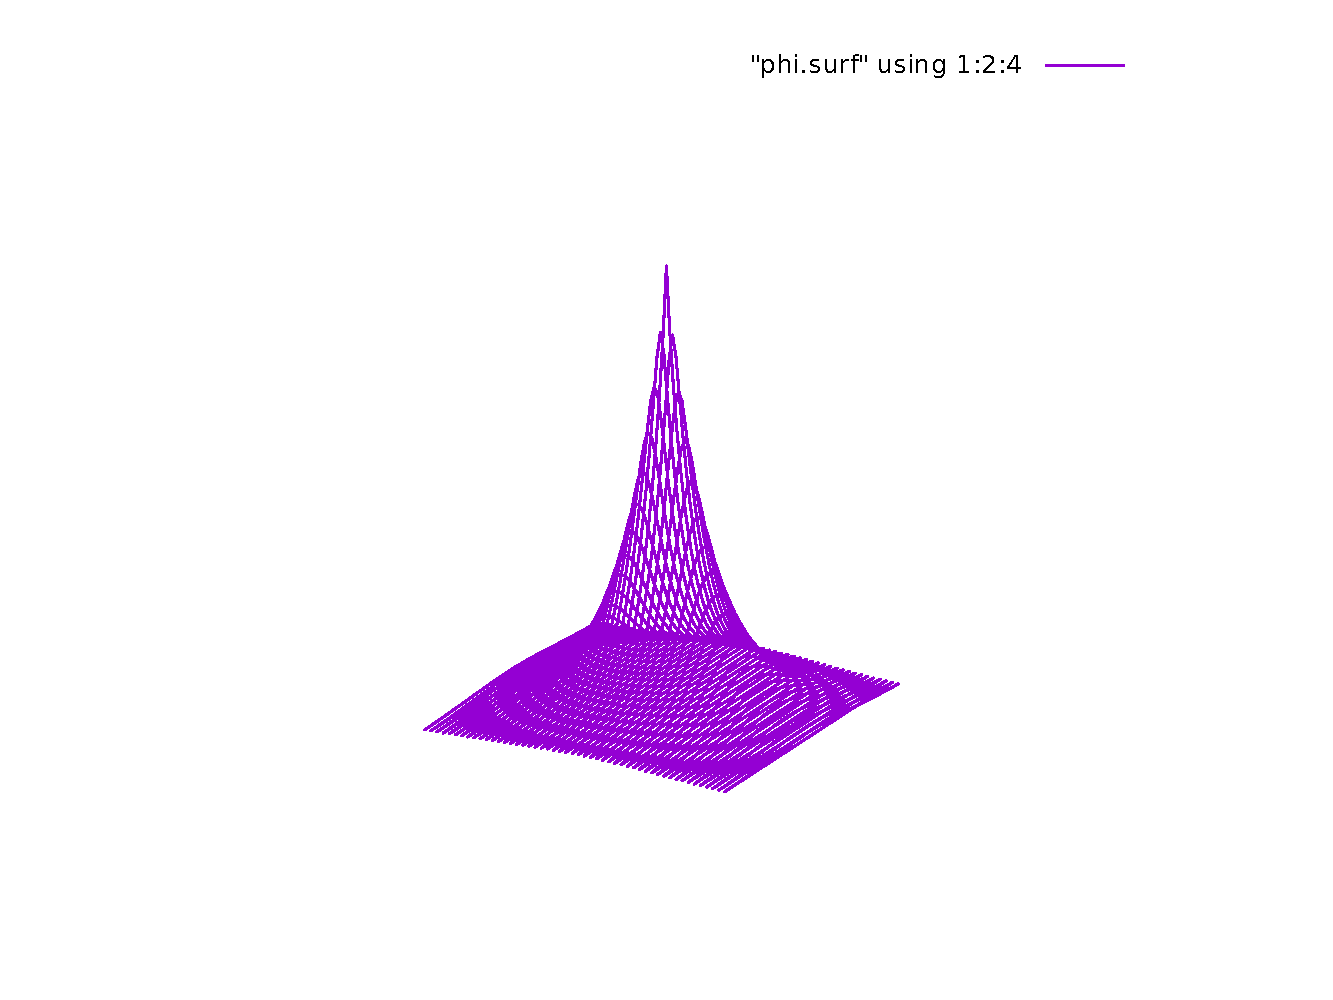
\includegraphics[scale=0.35, viewport = 175 90 430 400, clip]{figures/phi.pdf}
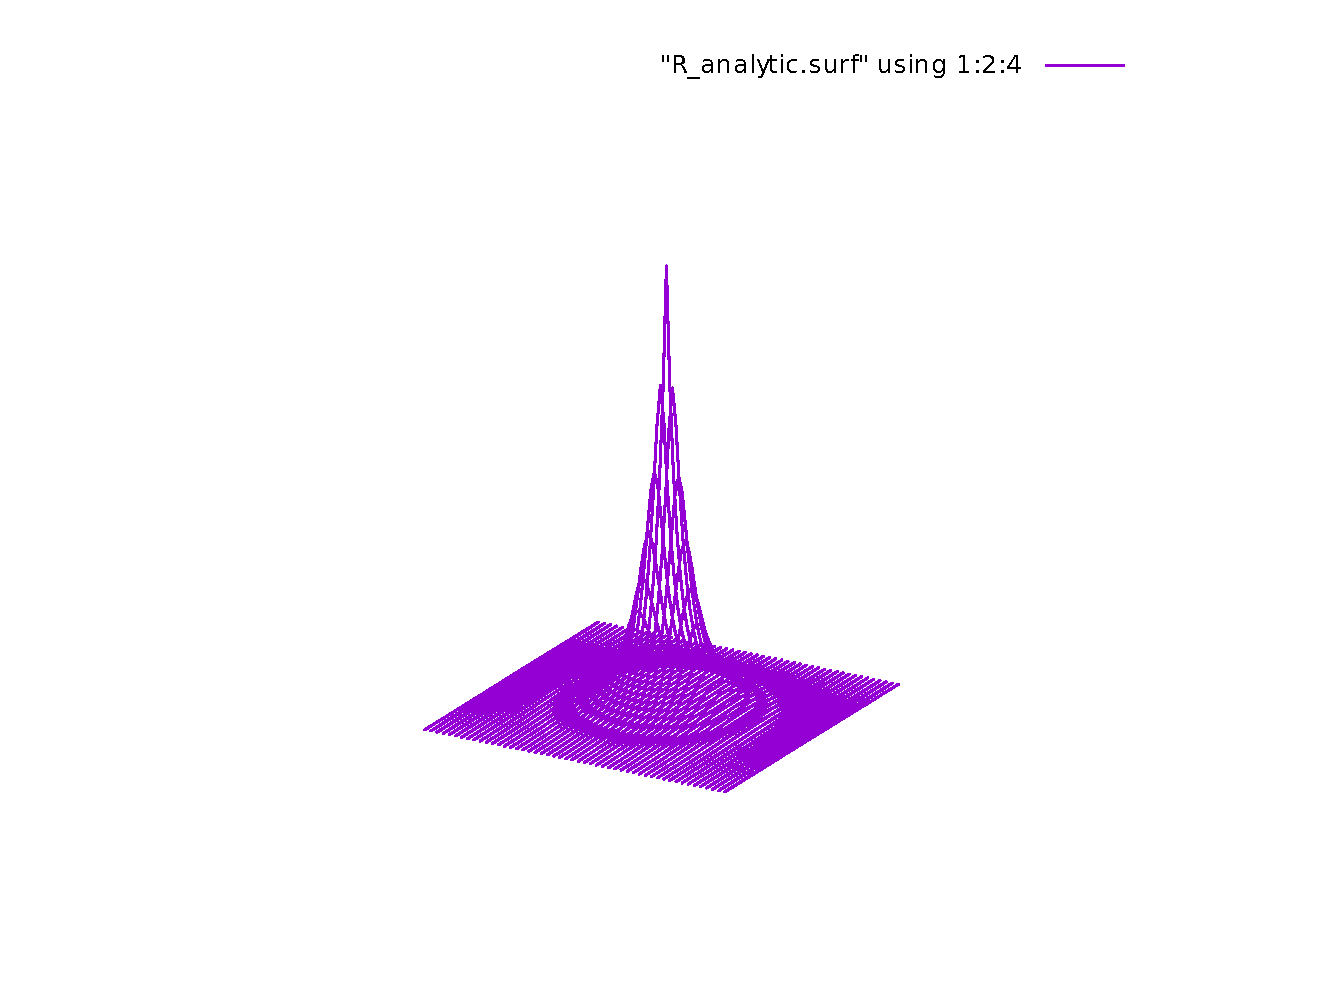
\includegraphics[scale=0.35, viewport = 175 90 430 400, clip]{figures/R.pdf}
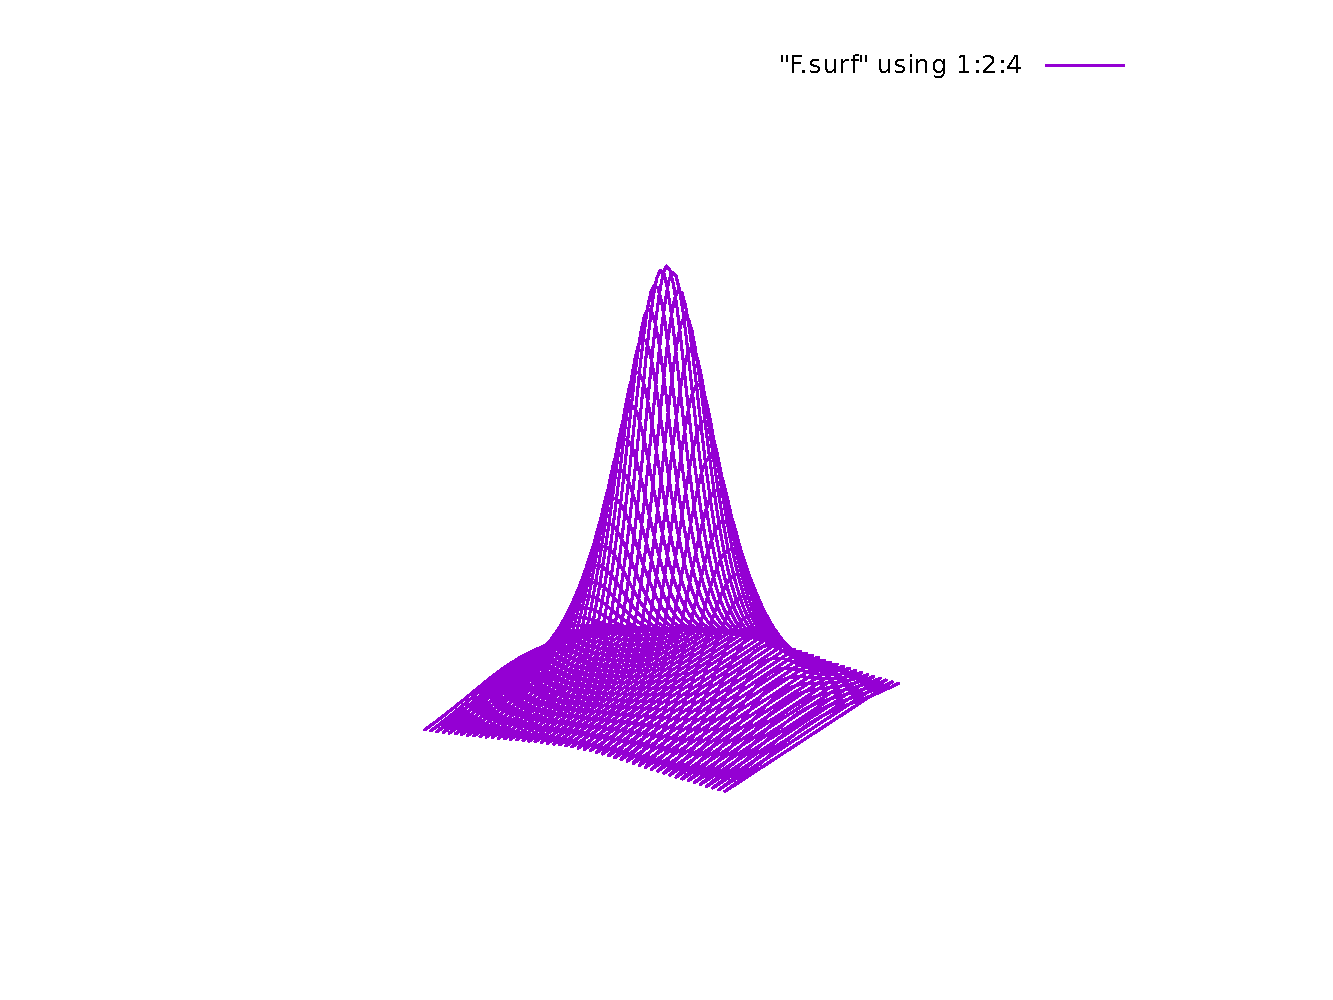
\includegraphics[scale=0.35, viewport = 175 90 430 400, clip]{figures/F.pdf}\\

\begin{table}
\begin{tabular}{ccccccc}
\hline
\hline
Precision&
\multicolumn{1}{c}{\ }&
\multicolumn{1}{c}{$\phi(r_0)$}&
\multicolumn{1}{c}{$\phi(r_1)$}&
\multicolumn{1}{c}{\ }&
\multicolumn{1}{c}{$\phi(r_0)$}&
\multicolumn{1}{c}{$\phi(r_1)$}\\
\hline
\hspace{5mm}\ &\hspace{1mm}\ &\hspace{15mm}\ &\hspace{15mm}\ &\hspace{2mm}\ &\hspace{15mm}\ &\hspace{15mm}\ \\
&\multicolumn{1}{c}{\ }
&\multicolumn{2}{c}{R = Identity}                          
&\multicolumn{1}{c}{\ }
&\multicolumn{2}{c}{R = Slater}\\                          
$\epsilon = 10^{-4}$ && \red{1.3e-02} & \yellow{6.3e-04}&& \green{2.4e-05}  & \yellow{1.6e-04}\\
$\epsilon = 10^{-5}$ && \red{4.3e-03} & \green{2.7e-06} && \green{4.6e-06}  & \green{2.4e-06} \\
$\epsilon = 10^{-6}$ && \red{1.4e-03} & \yellow{1.9e-06}&& \yellow{2.0e-06} & \green{8.8e-07} \\
$\epsilon = 10^{-7}$ && \red{6.4e-04} & \green{4.0e-08} && \green{6.7e-09}  & \green{1.9e-09} \\
$\epsilon = 10^{-8}$ && \red{1.1e-04} & \yellow{1.5e-08}&& \green{9.2e-10}  & \green{3.8e-09} \\
                     &&               &                 &&                  &                 \\
\hline
\hline
\end{tabular}
\end{table}

\centering
$r_0$ at the nucleus, $r_1$ at a random point away from the nucleus

\end{frame}

\begin{frame}
\frametitle{Similarity transform}
\scriptsize
Extension to many-electron systems

\end{frame}

\begin{frame}
\frametitle{Similarity transform}
\scriptsize
Methyloxirane convergence

\end{frame}
